\section{Introduction}

本書は初めてSCALE-LESモデルを利用するユーザー向けに,SCALE-LESモデルのインストールから実行までを解説したユーザーズガイドです.
本書中のシェルコマンド等はbash を想定して記述しています.異なる環境下では適宜読み替えて対応してください.
本書中の不明点やお気づきの点がございましたら\verb|****@riken.jp|(複合系気候科学研究チームの誰か)までご連絡ください.

\subsection{SCALEライブラリ}
SCALEとは''Scalable Computing for Advanced Library and Environment''の略であり,
理化学研究所 計算科学研究機構(AICS)を中心に開発が進められている次世代気象・気候科学における基盤ライブラリである.
Figure \ref{fig:scale}に示されるように,このライブラリは次世代のスーパーコンピュータから汎用計算機に至るまで広く用いられる事を念頭において開発されており,
気候・気象科学を専門とする科学者と計算機科学を専門とする科学者が共同で開発を行っている.

SCALEライブラリは京コンピュータをはじめとする並列計算機に対してチューニングされたモデルコンポーネントや
解析システム、およびテストセットや知見といった開発環境を提供することによって、
これらの問題を解決することを目的としている.
SCALEライブラリ(SCALE-LESモデルを含む)はBSD-2ライセンスにおいてフリーソフトウェアとして提供されており、
ユーザーの自由な利用・改変が許されている点も特徴といえる.

\begin{figure}[t]
\begin{center}
  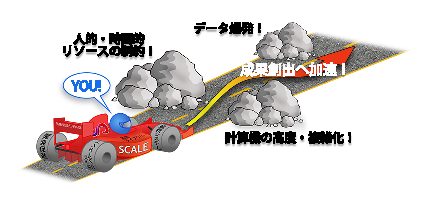
\includegraphics[width=0.6\hsize]{./figure/library.eps}\\
  \caption{SCALEライブラリのねらい}
  \label{fig:scale}
\end{center}
\end{figure}


\subsection{SCALEとSCALE-LESモデル}
SCALEライブラリを使用して構築された数値モデルの1例がSCALE-LESモデルである(Fig. \ref{fig:scale-les})。
格子系や力学コア,物理過程といったモデル構築に必要な基本的なコンポーネントはSCALEライブラリが提供するため、
SCALE-LESとして新たに用意されたのは、これらのコンポーネントをmanageするためのモデルドライバーや変数セットである。
SCALEライブラリをインストールしておくことで、SCALE-LESと同様な方法によってユーザーは新たなモデル作ることができる。

\begin{figure}[t]
\begin{center}
  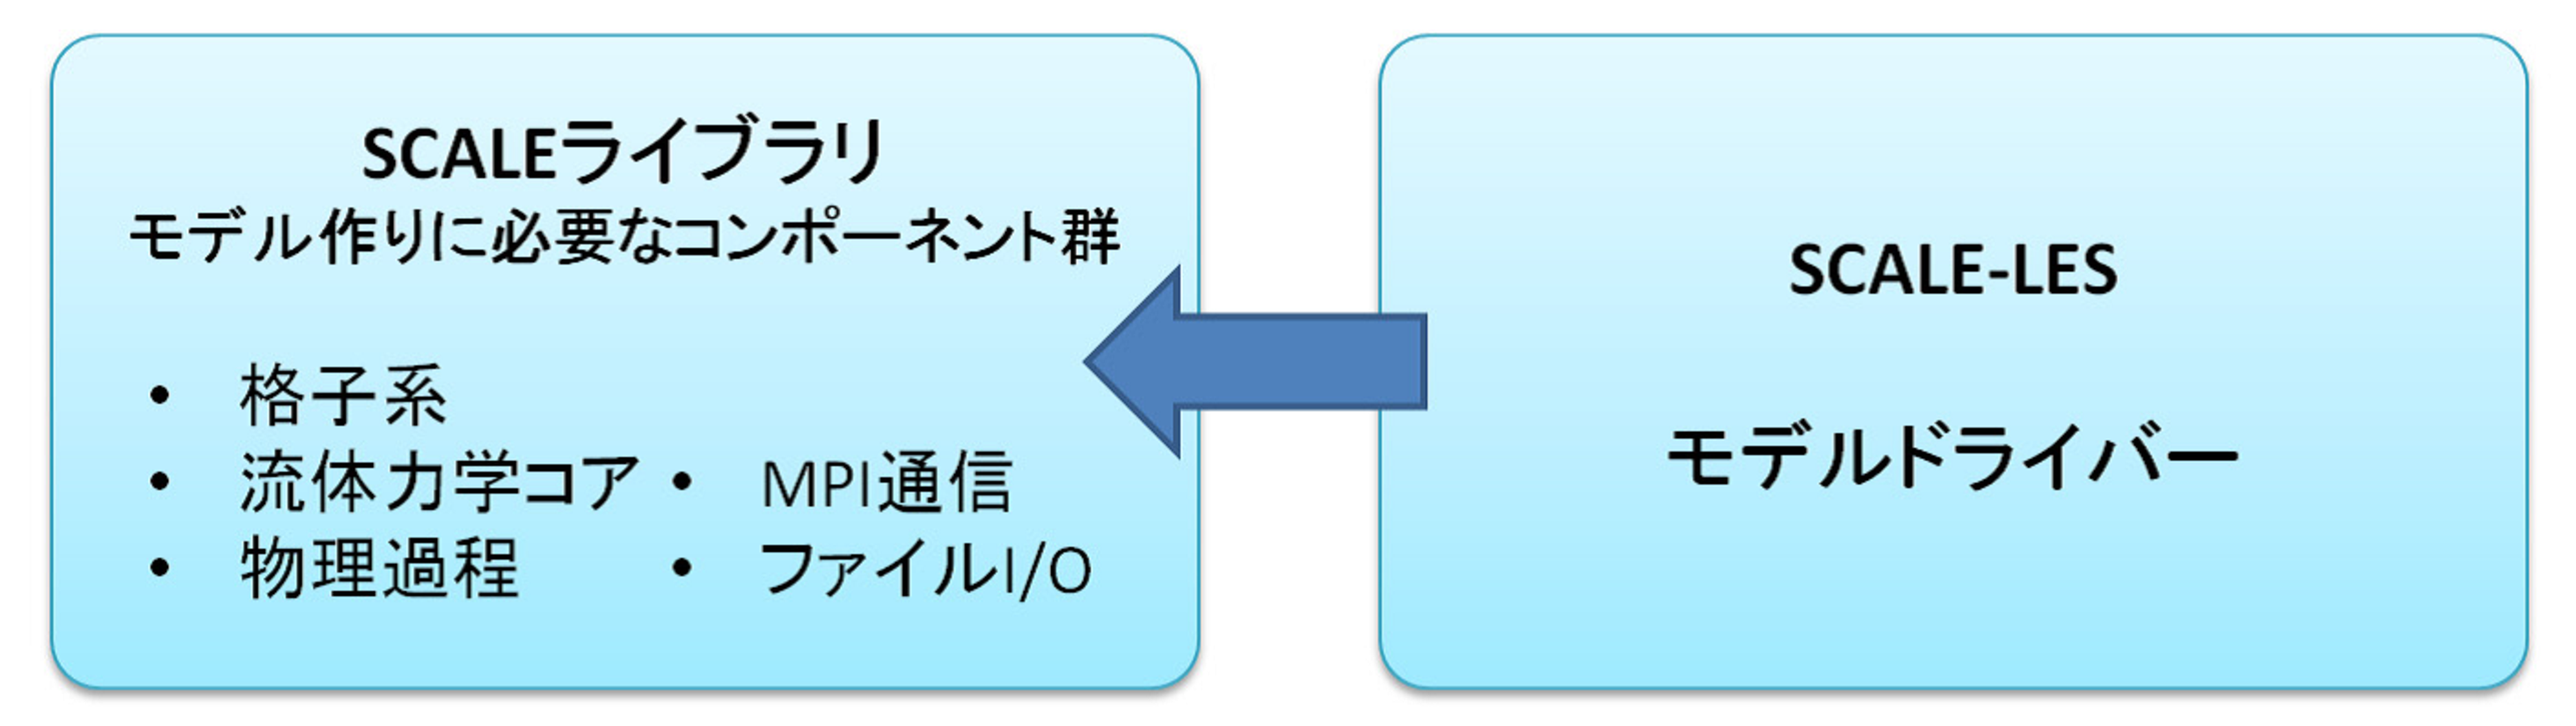
\includegraphics[width=0.9\hsize]{./figure/scale_and_scale-les.eps}\\
  \caption{SCALEライブラリとSCALE-LESモデルの関係}
  \label{fig:scale-les}
\end{center}
\end{figure}


\subsection{SCALE-LESモデルの構成}
詳細なモデル構成や差分化手法については,Sato et al. (2014) を参照されたい.
現在,SCALE-LESモデルとして組み込まれているコンポーネントは下記のものである.

{\bf フレームワーク関係}
\begin{itemize}
\item Cartesian グリッドシステム(Arakawa C-grid)
\item Cartesian ベースMPI通信
\item Map-projection \& Map-factors
\item Nestingシステム(1-way, offline, and online)
\item gtoolベースnetcdf4ファイル I/O
\item WRF-ARW,NICAM向け外部データ読み込み
{\bf 力学コア関係}
\item 方程式系: 3次元完全圧縮流体方程式
\item 数値解法:HE-VE,  HE-VI,HI-VIスキームから選択可能
\item 空間差分:4次中央差分
\item 時間差分:3次ルンゲクッタスキーム
\item 非負保証:FCTスキーム
\item 数値フィルター:4次Hyper diffusion
\item 地形:Terrain-followingスキーム
{\bf 物理過程}
\item 乱流過程:Smagorinsky typeのサブグリッドモデル, MYNN2.5境界層モデルから選択可能
\item 雲微物理:Kessler type バルクモデル(Kessler 1969),6-class single moment バルクモデル(tomita 2006),6-class double moment バルクモデル(Seiki and Nakajima 2014),ビン法雲モデル(Suzuki et al. 2010)から選択可能
\item 放射過程:MSTRN-X (Sekiguchi and Nakajima 2008)
\item 陸面モデル:バケツモデル(Louis 1994,Beljoursから選択可能)
\item 海洋モデル(スラブモデル)
\item 都市キャノピーモデル
\end{itemize}

上記に加えて,SCALE-LESモデル本体のドライバー、現実事例の計算に必要な地形や土地利用データを作成するツール、
理想実験の初期値・境界値、もしくは外部モデルから初期値・境界値を作成するツールが提供されている。

なお、本ユーザーズガイド内の説明で、コマンドラインのシンボル(\verb|$|)があれば、コマンドの実行を示す.
